\documentclass[12pt,a4paper]{article}

\usepackage[english]{babel}
\usepackage{listings}
\usepackage{ucs}
\usepackage{color}

%%%%% LAY OUT %%%%%%
\linespread{1.2}
\usepackage[margin=1in]{geometry}
\usepackage{tabularx}
\usepackage{fancyhdr}
\usepackage{verbatim}
\usepackage{enumerate}
\usepackage{sectsty}								
\allsectionsfont{}	% Change font of al section commands


\pagestyle{fancy}
\lhead{}
\rhead{\nouppercase{\leftmark}}
\lfoot{}
\rfoot{}
\cfoot{\thepage}
\renewcommand{\headrulewidth}{0.4pt}
\renewcommand{\footrulewidth}{0.4pt}

\usepackage{graphicx}

%%%%% MATH %%%%%
\usepackage{amsmath}
\usepackage{amsthm}
\usepackage{multirow}
\usepackage{mathtools}	
\usepackage{wasysym}
\usepackage{amssymb}
\usepackage{amscd}
\usepackage{xfrac}
\numberwithin{equation}{section}




\newtheorem{theorem}{Theorem}
\newtheorem{lemma}{Lemma}
\newtheorem{corollary}{Corollary}

\usepackage{dsfont}
\usepackage{bm}

\usepackage{titlesec}

\newcommand{\p}[1]{\mathds{P}\left\{#1\right\}}

\begin{document}

\title{Allele frequency estimation under alignment and typing uncertainty \\ A general latent variable framework for genotyping, de novo and somatic mutation calling}
\author{Louis Dijkstra\footnote{E-mail: \texttt{dijkstra@cwi.nl}}}

\maketitle

\begin{abstract}
	 
\end{abstract}


\section{Introduction} \label{sec:introduction}

% Estimating the frequency with which a certain genetic variant occurs in a population is of importance for a large number of studies
% Often done on the basis of next-generation sequence data
% Although its merits, this type of data suffers from a number of sources of uncertainty that obscure the genetic signal 
% Two uncertainties that we want to take into account
% 1) alignment uncertainty 
% 2) typing uncertainty 
% Current approach: take the most likely one and discard the rest -> not a good approach
% Method that takes 

\subsection{(Next-generation) sequence data}

% Paired-end reads

% Two types of alignments to a certain indel of interest
% Internal segment alignment
% Overlapping alignment (split-reads) 

% Alignment likelihoods are given by the aligner

\subsection{Notation and nomenclature}

Manifest and latent variables are denoted with, respectively, Latin capital letters and Greek symbols. Observations/realizations of manifest variables are represented by a small letter. 

\section{The general model}

In this section we present a (Bayesian) latent variable model that links (next-generation sequence) reads and their alignments with the allele frequency of a variant of interest. We made the choice for a latent variable model for mainly two reasons: 
\begin{enumerate}
	\item the allele frequency is a quantity that cannot be observed directly and representing it, therefore, as a hidden/latent variable seems to be natural; 
	\item a latent variable model allows for incorporating measurement uncertainties in a clear way [REF]. 
\end{enumerate}

\begin{figure}
	\centering
	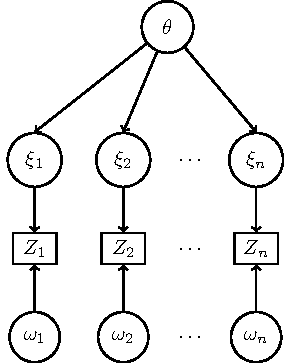
\includegraphics[width=0.3\textwidth]{general_latent_variable_model.pdf}
	\caption{The general latent variable model. Latent variables are shown with circles, while manifest variables are represented by boxes. }
\end{figure}

\paragraph{The variant allele frequency (VAF)}

Let $\theta \in \Theta \subset [0,1]$ be a latent random variable representing the main quantity of interest: the variant allele frequency (\textsc{vaf}) of a particular indel. We will assume that the locus of the indel is given beforehand and that its length, denoted by $\delta$, is known. We will for the moment assume a little as possible about $\theta$: its supports can either be discrete\footnote{In the case of a diploid individual, for example, the support of the \textsc{vaf} is $\Theta = \{0, \sfrac{1}{2}, 1\}$, since none, only one or both of the chromosomal copies can harbour the variant allele.} or continuous (which will depend on the application at hand, see Sect. XXX). In addition, we assume a uniform (hyper-)prior: 
\begin{equation}
	\theta \sim \text{uniform over }\Theta.  
\end{equation}

\paragraph{Alignments}
Let $R = \{R_1, R_2, \dots, R_n\}$ be a sequence of reads and $A = \{A_1, \dots, A_n\}$ be the corresponding set of alignments to the locus of interest provided by an aligner. Each alignment is associated with an \emph{alignment probability} denoted with $\pi_i$, i.e., the chance that alignment $A_i$ is the origin of the $i$-th read. 

Let $Z' = \left(Z_1, Z_2, \dots, Z_n \right) \in \mathds{R}^n$ be a vector of manifest variables representing observed quantities derived from $n$ different alignments, i.e., 
\begin{equation}
	Z_i := w_i\left(A_i\right) \qquad \text{for }i = 1,2\dots,n. 
\end{equation}
We will for the moment not specify the functions $w_i(\cdot)$; this depends on the type of read and how it is aligned to the locus of interest. For now we will limit ourselves to describe how these observations can be linked to our original quantity of interest, the \textsc{vaf} $\theta$. We do this to show how the model presented here can be easily adapted to accomodate a wide variety of reads/alignments and observations. Later on we will show how the measurement model can applied specifically to internal segment lengths and overlapping alignments. 

As mentioned before, any observation based on an alignment is commonly associated with two types of uncertainty: 1) alignment uncertainty (the alignment could be placed erroneously), and 2) typing uncertainty (the alignment can only support the presence/absence of a genetic variant up to a certain level). These two types of uncertainties are represented in our model by associating every observation $Z_i$ with two Bernoulli distributed latent variables: $\omega_i$ and $\xi_i$. The latent variable $\omega_i$ is $1$ iff the $i$-th alignment is placed correctly and $0$ otherwise. The probability of alignment $i$ to be correctly aligned is commonly provided by the aligner and denoted here with $\pi_i$: 
\begin{equation}
	\omega_i \sim \text{Bernoulli}\left(\pi_i \right) \qquad \text{for }i=1,2\dots,n.
\end{equation}
Note that when an alignment $Z_i$ only provides information about $\theta$ when it stems from the locus of interest, i.e., $\omega_i = 1$. The binary variable $\xi_i$ is $1$ iff the $i$-th alignment stems from a chromosome that harbours the indel of interest and $0$ otherwise. The probability that a read stems from a variant-allele-affected chromosome is equal to the variant allele frequency\footnote{Or at least, under the assumption that a chromosome carrying the indel is equally likely to bring forth a read as a chromosome not harboring the indel.}, $\theta$, i.e.,
\begin{equation}
	\xi_i \mid \theta \sim \text{Bernoulli}\left(\theta  \right) \qquad \text{for }i=1,2\dots,n.
\end{equation}
Whether $\xi_i$ is $1$ or $0$ is often not evident from the value of $Z_i$, although the values $Z_i$ is likely to take will vary when the indel is present or not. More formally, 
\begin{equation}
	\begin{aligned}
	Z_i \mid \omega_i = 1, \xi_i = 0 & \sim f_i^{(\text{absent})} \\ 
	Z_i \mid \omega_i = 1, \xi_i = 1 & \sim f_i^{(\text{present})} \\ 
	\end{aligned}
\end{equation}
for $i = 1,2,\dots,n$. The probability distributions $f_i^{(\text{absent})}$ and $f_i^{(\text{present})}$ returns the probability of observing a certain realization $Z_i$ when the indel of interest is either absent or present. When the $i$-th alignment does not stem from the locus of interest, i.e., $\omega_i = 0$: 
\begin{equation}
	Z_i \mid \omega_i = 0 \sim u_i \qquad \text{for }i = 1,2\dots,n. 
\end{equation}
The probability distribution $u_i$ is arbitrary and should be chosen such that the posterior distribution of the \textsc{vaf} $\theta$ is not influenced. We will return to this point later. 

The probability distribution of $Z_i$ given the \textsc{vaf} $\theta$, $g_i(z_i \mid \theta)$, can easily be found by applying the law of total probability repeatedly: 
\begin{equation}
	\begin{aligned}
		g_i (z_i \mid \theta) & =  g_i (z_i \mid \theta, \omega_i = 1) \p{\omega_i = 1} + g_i (z_i \mid \theta, \omega_i = 0) \p{\omega_i = 0} \\
					& = \pi_i g_i (z_i \mid \theta, \omega_i = 1) + \left(1 - \pi_i \right) u_i (z_i).
	\end{aligned}
\end{equation}
The probability distribution $g_i (z_i \mid \theta, \omega_i = 1)$ is given by
\begin{equation}
	\begin{aligned}
		g_i (z_i \mid \theta, \omega_i = 1) 	& = g_i (z_i \mid \theta, \omega_i = 1, \xi_i = 1) \p{\xi_i = 1 \mid \theta} \\ 
							& +  g_i (z_i \mid \theta, \omega_i = 1, \xi_i = 0) \p{\xi_i = 0 \mid \theta} \\
							& = \theta f_i^{\text{(present)}}(z_i) + (1 - \theta) f_i^{\text{(absent)}}(z_i).
	\end{aligned}
\end{equation}
In conclusion, 
\begin{equation}
	g_i (z_i \mid \theta) = \pi_i \left[\theta f_i^{\text{(present)}}(z_i) + \left(1 - \theta \right) f_i^{\text{(absent)}}(z_i) \right] + \left(1 - \pi_i \right) u_i(z_i). 
\end{equation}


\paragraph{The posterior distribution of the VAF $\theta$}

The posterior distribution of the \textsc{vaf} $\theta$ is given a vector of observations $z$:
\begin{equation}
	h(\theta \mid Z) = \frac{f(z \mid \theta) h(\theta)}{f(z)} \qquad \text{(Bayes' rule)} 
\end{equation} 
where $f(z \mid \theta)$ is the likelihood of the data given $\theta$, $h(\cdot)$ is the \textsc{vaf}'s (uniform) prior and $f(z)$ is 
$\sum_{\theta \in \Theta} f(z \mid \theta) h(\theta)$ and $\int_{\theta \in \Theta} f(z \mid \theta) h(\theta) d\theta$, when the support of $\theta$ is, respectively, discrete and continuous. Under the assupmtion of local/conditional independence of the manifest variables $Z_1, Z_2, \dots, Z_n$, the likelihood is linear in the number of aligments: 
\begin{equation}
	\begin{aligned}
	L(\theta \mid z)& = f(z_1, z_2, \dots, z_n \mid \theta)  \\ 
			& = \prod_{i = 1}^n g_i (z_i \mid \theta) \\
			& = \prod_{i = 1}^n \left\{\pi_i \left[\theta f_i^{\text{(present)}}(z_i) + \left(1 - \theta \right) f_i^{\text{(absent)}}(z_i) \right] + \left(1 - \pi_i \right) u_i(z_i) \right\}.
	\end{aligned}
\end{equation}
Note that the likelihood function is a $n$-degree polynomial in $\theta$. Determining its maximum analytically when $\theta$'s support is continuous, is, therefore, impossible. 



\begin{theorem}
	The likelihood function $L(\theta \mid z_1, \dots, z_n)$ attains a unique global maximum $\widehat{\theta}$ on the unit interval $\Theta = [0,1]$ when (1) the subset 
	\begin{equation}
		I := \{\theta \in \Theta: g_i(z_i \mid \theta) > 0 \text{ for } i =1,\dots,n\}
	\end{equation}
	is connected and non-empty, and, (2) there exists an observation $z_i$ for which the alignment probability $\pi_i$ is strictly larger than zero and $f_i^{\text{(present)}}(z_i) \neq f_i^{\text{(absent)}}(z_i)$. 
\end{theorem}
\begin{proof}
Note that $L(\theta \mid z_1, \dots, z_n) = \prod_i g_i(z_i \mid \theta) = 0$ when $\theta \not\in I$, since for those $\theta$'s there exists an observation $z_i$ for which the likelihood $g_i(z_i \mid \theta)$ is equal to zero. The likelihood $L(\theta \mid z_1, \dots, z_n)$ is strictly larger than zero by definition when $\theta \in I$. Since the likelihood function is a $n$-th order polynomial and, therefore, continuous, it must attain a global maximum on the interval $I$. 

Suppose condition \emph{(1)} is met. The point $\widehat{\theta} \in I$ is a maximum of $L(\cdot \mid z_1, \dots, z_n)$ if and only if it is a maximum of the loglikelihood function 
\begin{equation}
	\ell(\theta \mid z_1, \dots, z_n) := \log L(\theta \mid z_1, \dots, z_n) = \sum_{i=1}^n \log g_i(z_i \mid \theta) \qquad (\theta \in I)
\end{equation}
since the logarithm is a monotonic transformation. Note that the loglikelihood function is only defined on the subset $I$. The second order derivative of the loglikelihood with respect to the \textsc{vaf} is easily found to be
\begin{equation}
	\frac{\partial^2 \ell}{\partial \theta^2} = - \sum_{i = 1}^n \left[\frac{\partial g_i(z_i \mid \theta) / \partial \theta}{g_i(z_i \mid \theta)} \right]^2 \leq 0
\end{equation}
 indicating that the loglikelihood function is concave. Note that it is strictly concave, i.e., $\partial^2 \ell / \partial \theta^2 < 0$, iff there exists an observation $z_i$ for which
\begin{equation}
	\frac{\partial g_i(z_i \mid \theta)}{\partial \theta} = \pi_i \left[f_i^{\text{(present)}}(z_i) - f_i^{\text{(absent)}}(z_i) \right] \neq 0.
\end{equation}
This inequality holds only when $\pi_i \neq 0$ and $f_i^{\text{(present)}}(z_i) \neq f_i^{\text{(absent)}}(z_i)$ which constitutes condition \emph{(2)}. 

Suppose $I$ is a non-empty closed set on the unit interval, i.e., $I = [a,b]$. Since the loglikelihood is strictly concave when condition \emph{(2)} is met, it attains a unique global maximum $\widehat{\theta}$ on $I$. Because the logarithm is a monotonic transform, $\widehat{\theta}$ must be the unique global maximum of the likelihood function as well. 

A similar reasoning holds up when $I$ is open or half-open. The maximum must lie in the interior of $I$, since the likelihood function is zero for those endpoints not in $I$, e.g., when $I$ is the open interval $(a,b)$, $L(a \mid z_1, \dots, z_n) = L(b \mid z_1, \dots, z_n) = 0$ while $L(\theta \mid z_1, \dots, z_n)$ is strictly positive on $I$. The loglikelihood function is strictly concave on $I$, therefore, the likelihood function attains a unqiue global maximum. \qedhere 
\end{proof}


The functions $u_i(\cdot)$ must be chosen such that
\begin{enumerate}
 \item when $\pi_i = 0$, i.e., the read in question does with 100\% certainty not align to the locus of interest, then the observation $z_i$ should not provide any information on the \textsc{vaf} $\theta$, i.e., $h(\theta \mid z_i) = h(\theta)$. 
\end{enumerate}
The first condition is met for any probability distribution $u_i(\cdot)$ that does not depend on $\theta$, since the posterior distribution $h(\theta \mid z_i)$ when $\pi_i = 0$ is equal to
\begin{equation}
 h(\theta \mid z_i) = \frac{u_i(z_i) h(\theta)}{\int_\Theta u_i(z_i) h(\theta) d\theta} = \frac{u_i(z_i) h(\theta)}{u_i(z_i) \int_\Theta h(\theta) d\theta} = h(\theta). 
\end{equation}
(The derivation is similar when the support of $\theta$ is discrete).

% Bayesian model for describing the data
% Introduce VAF. Support is either discrete or continuous depended on the application (see Section ...)

\subsection{Alignments}

Let $Z \in \mathds{R}$ be a manifest variable denoting an observation based on an alignment. Every alignment is surrounded with uncertainty.  

\subsubsection{Internal segments: an alternative mixture model}

% Internal segment lengths are thought to follow approximate a Normal distribution. We will use: 
% f_lambda(x) etc. 

% Unclear where an alignment stems from. A latent mixture model! 

% Extension with alignment uncertainty 

\subsubsection{Overlapping alignments}

\subsection{The full latent variable model}

\subsection{Posterior distribution of the VAF}

\subsection{Continuous support}

\subsection{Likelihood ratio based confidence intervals}

\subsection{Comparing evidences: internal segment vs. overlapping alignments}

\section{Applications \& Extensions}

\subsection{Genotyping: the di- and polyploid case}

\subsection{DeNovo mutation calling}

\subsection{Somatic mutation calling}


\end{document}
